\documentclass[a4paper,  11pt]{ctexart}
\usepackage{srcltx,graphicx}
\usepackage{amsmath, amssymb, amsthm}
\usepackage{color}
\usepackage{lscape}
\usepackage{multirow}
\usepackage{psfrag}
\usepackage{diagbox}
\usepackage[hang]{subfigure}
\usepackage{float}
\usepackage[colorlinks,linkcolor=black,anchorcolor=blue,citecolor=green]{hyperref}

\newtheorem{theorem}{Theorem}
\newtheorem{lemma}{Lemma}
\newtheorem{definition}{Definition}
\newtheorem{comment}{Comment}
\newtheorem{conjecture}{Conjecture}

\newcommand\bbR{\mathbb{R}}
\newcommand\bbN{\mathbb{N}}
\newcommand\bbC{\mathbb{C}}
\newcommand\bx{\boldsymbol{x}}
\newcommand\dd{\,\mathrm{d}}

\newcommand\diag{\mathrm{diag}}
\newcommand\tr{\mthrm{tr}}

\setlength{\oddsidemargin}{0cm}
\setlength{\evensidemargin}{0cm}
\setlength{\textwidth}{150mm}
\setlength{\textheight}{230mm}

\newcommand\note[2]{{{\bf #1}\color{red} [ {\it #2} ]}}
%\newcommand\note[2]{{ #1 }} % using this line in the formal version

\newcommand\pd[2]{\dfrac{\partial {#1}}{\partial {#2}}}
\newcommand\od[2]{\dfrac{\dd {#1}}{\dd {#2}}}
\newcommand{\bm}[1]{\mbox{\boldmath{$#1$}}}

\begin{document}
\title{图像处理中的数学方法-homework1}
\author{郑灵超}
\maketitle
%\tableofcontents
%\newpage

\section{作业一}
\subsection{一阶偏导数}
根据课程PPT第77页内容,左图对应的导数为
\[
\pd{v}{x}\Big|_{i,j} = \frac{\lambda}{2} + 
\frac{1-\lambda}{2}=\frac{1}{2},\quad 
\pd{v}{y}\Big|_{i,j}=0,
\]
而右图对应的数值格式,
\[
\pd{v}{x}\Big|_{i,j}=\pd{v}{y}\Big|_{i,j}=
\frac{\lambda}{2}+\frac{1-\lambda}{2}\frac{1}{2}=\frac{1+\lambda}{4},
\]
因此当$\lambda=\sqrt{2}-1$时,二者离散导数的模相同。
\subsection{拉普拉斯算子}
根据课程PPT第78页内容,左图对应的数值格式的拉普拉斯算子为
\[
\Delta v|_{i,j}= \lambda + 1-\lambda = 1,
\]
右图对应的数值格式的拉普拉斯算子为
\[
\Delta v|_{i,j}= 2\lambda+\frac{1-\lambda}{2}=
\frac{1+3\lambda}{2},
\]
因此当$\lambda=\frac{1}{2}$时,二者拉普拉斯的值相同。
\section{作业二}
\subsection{问题介绍}
对模型进行去噪去模糊,本次我们采用的模型为 
\begin{equation}
    \label{eq:model}
    \hat{u}=\mathop{\arg\min}_u \lambda \int \vert \nabla u \vert
    \text{d} x + \frac
    12\int(Au-f)^2 \text{d}x,
\end{equation}
其中$A$是用于模拟图像模糊的卷积矩阵,卷积核为
\[
k = \text{fspecial}("Gaussian",[15,15],\sigma_1),\sigma_1=1.5,2.
\]
假设原图为$\tilde{u}$,待处理的图像可以由如下方式生成:
\[
  f =
  A\tilde{u}+\sigma_2\text{randn},\sigma_2=\frac{\max(\tilde{u})}{100}
  ,\frac{\max(\tilde{u})}{200}.
\]

\subsection{问题分析}
\subsubsection{算法介绍}
我们采用的算法为ADMM算法,其迭代格式如下:
\begin{enumerate}
    \item $u_{k+1}=(A^TA+\mu W^TW)^{-1}(A^Tf+\mu W^T(d_k-b_k)),$
    \item $d_{k+1}=\mathcal{T}_{\bm\lambda/u}(Wu_{k+1}+b_k),$
    \item $b_{k+1}=b_k+\delta(Wu_{k+1}-{k+1}).$
\end{enumerate}
迭代的终止条件为
\[
\frac{\Vert Wu_{k+1}-d_{k+1}\Vert_2 }{\Vert f\Vert_2}<tol.
\]
\subsubsection{算法分析}

算子$A$对应于一个矩阵$A$与$f$的卷积,算子$W^TW$对应于矩阵$L$与$f$的卷
积,
记$\hat{A},\hat{L},\hat{f}$分别为它们的Fourier变换后的矩阵,则迭代格式第一步等
价于

\[
    (\hat{A}*\hat{A}+\mu\hat{L})*\hat{u}_{k+1}=\hat{A}*\hat{f}+\mu
    (W^T(d_k-b_k))^{\hat{} }.
\]
而为了求解迭代过程中的第一个方程,我们采用FFT算法,步骤如下:
其中这里的$*$表示矩阵逐分量相乘。\par
因此我们可以通过如下步骤求解该方程:
\begin{enumerate}
    \item 计算算子$A^TA$和$W^TW$的Fourier变换的矩阵$\hat{A}$与
        $\hat{\Delta}$,以及$\hat{f}$和$W^T(d-b)$的Fourier变换
        $\hat{v}$.
    \item 计算$
        (\hat{A}*\hat{f}+\mu\hat{v})/(\hat{A}*\hat{A}+\mu\hat{L})$,
        这里的$*,/$均表示逐项操作。
    \item 做Fourier逆变换得到$u$.
\end{enumerate}


\subsection{实验结果}

我们使用了经典的Lena图作为实验图片,对其进行加噪声与模糊得到待处理图片
,再利用之前的算法进行去噪去模糊,得到的结果如下:

\begin{figure}[H]
    \centering
    \subfigure{
    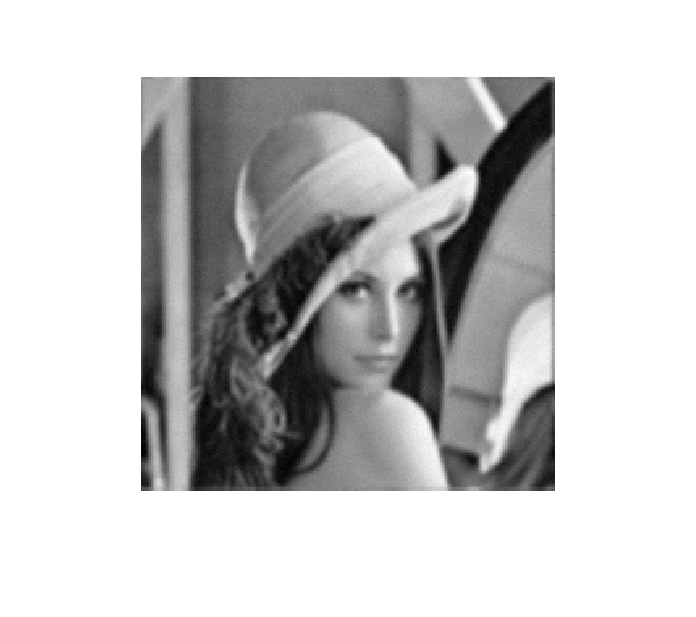
\includegraphics[width=0.45\textwidth]{../program/Lenna-1.eps}}
    \subfigure{
    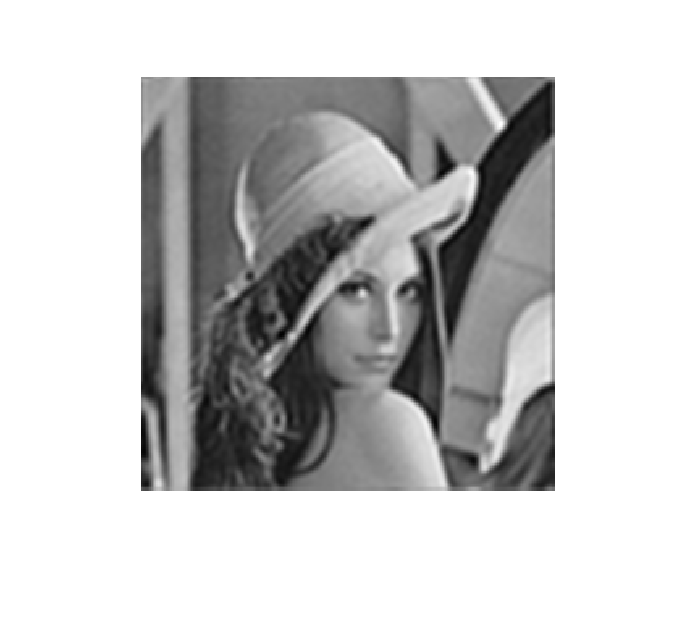
\includegraphics[width=0.45\textwidth]{../program/Lenna-2.eps}}
    \caption{$\sigma_1=1.5,\sigma_2=|u|/100$}
\end{figure}
\begin{figure}[H]
    \centering
    \subfigure{
    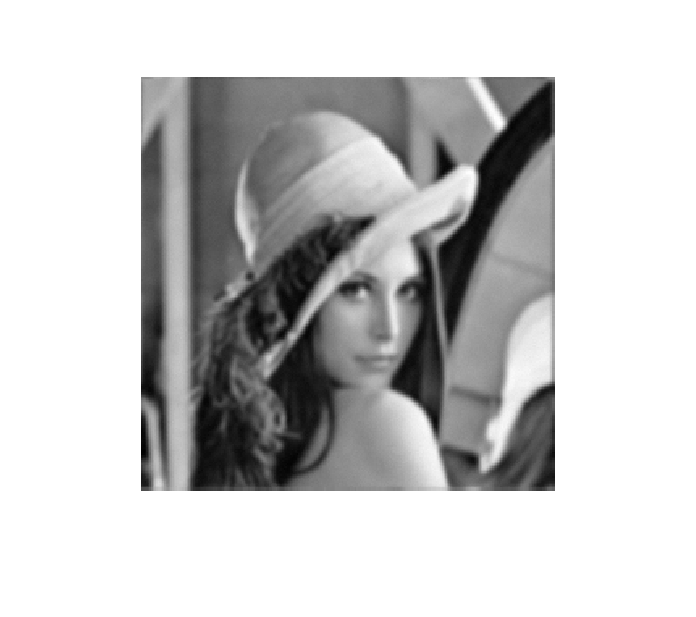
\includegraphics[width=0.45\textwidth]{../program/Lenna-3.eps}}
    \subfigure{
    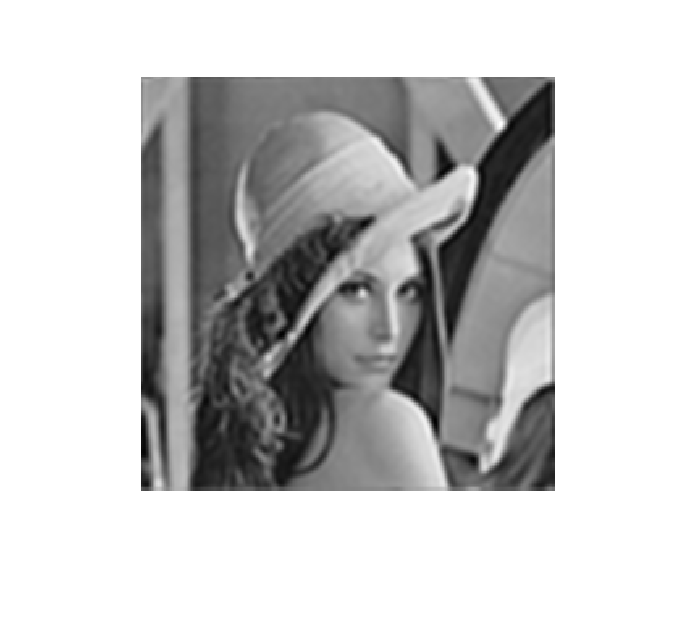
\includegraphics[width=0.45\textwidth]{../program/Lenna-4.eps}}
    \caption{$\sigma_1=1.5,\sigma_2=|u|/200$}
\end{figure}
\begin{figure}[H]
    \centering
    \subfigure{
    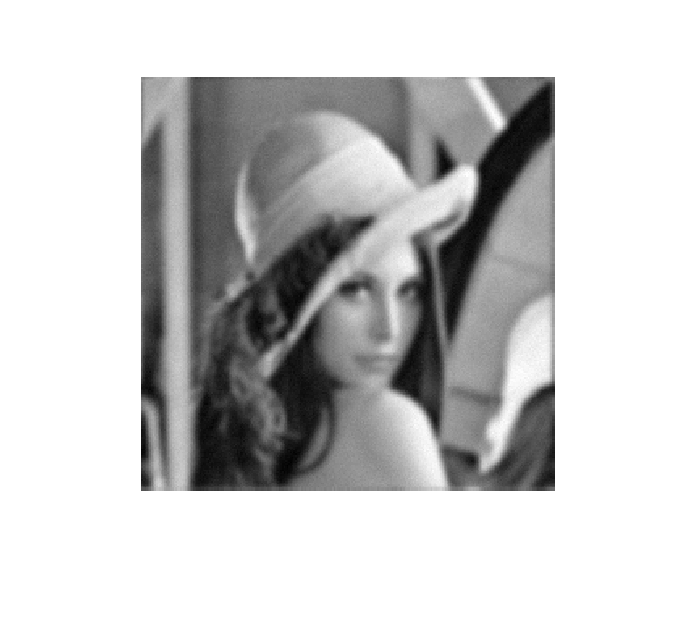
\includegraphics[width=0.45\textwidth]{../program/Lenna-5.eps}}
    \subfigure{
    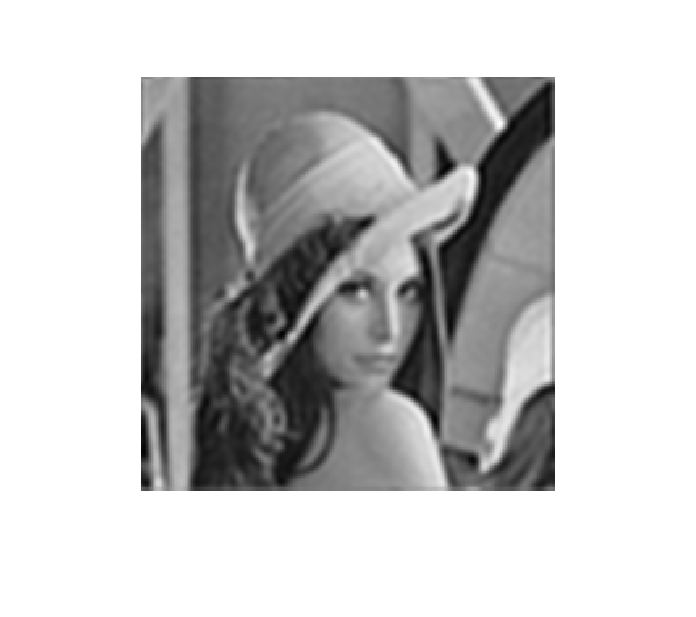
\includegraphics[width=0.45\textwidth]{../program/Lenna-6.eps}}
    \caption{$\sigma_1=2,\sigma_2=|u|/100$}
\end{figure}

\begin{figure}[H]
    \centering
    \subfigure{
    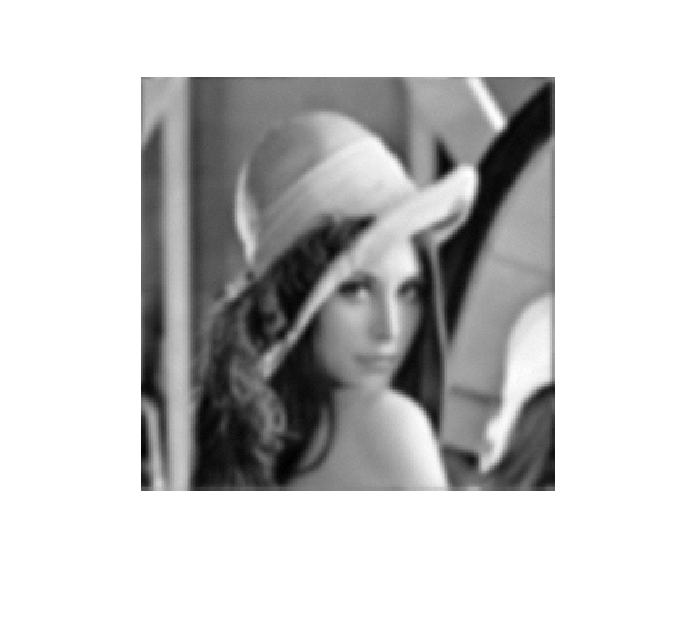
\includegraphics[width=0.45\textwidth]{../program/Lenna-7.eps}}
    \subfigure{
    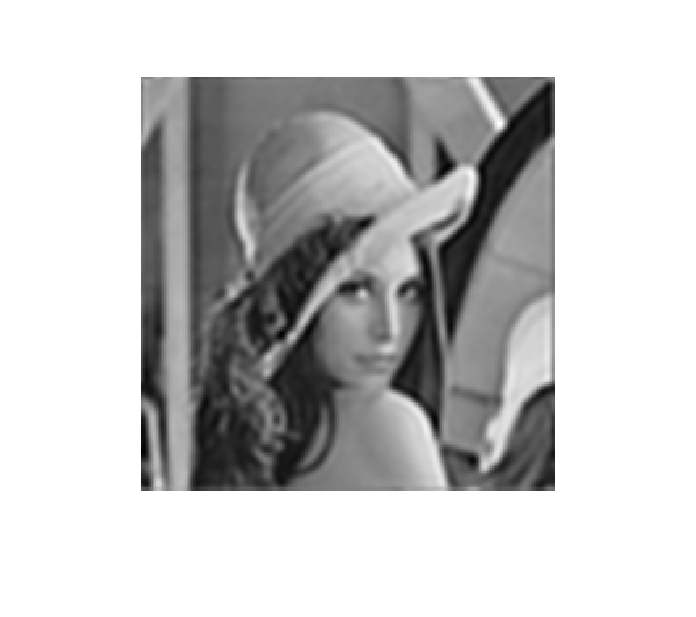
\includegraphics[width=0.45\textwidth]{../program/Lenna-8.eps}}
    \caption{$\sigma_1=2,\sigma_2=|u|/200$}
\end{figure}
而关于原图的相对误差,得到的结果如下:
\begin{table}[H]
    \centering
    \begin{tabular}{|c|c|c|}
        \hline
        \diagbox{$\sigma_1$}{$err$}{$\sigma_2$} & 100 & 200 \\
        \hline
        1.5 & 0.0234 & 0.0235\\
        \hline
        2 &  0.0261 & 0.0262 \\
        \hline 
    \end{tabular}
\end{table}
以上实验的参数选取为
$\mu=1,\lambda=0.01,\delta=0.1,maxstep=100,tol=1e-7$。\par
其中加了噪声与模糊而未进行去噪的误差,当$\sigma_1=1$时为0.026,当
$\sigma_1=2$时为0.032。可见该去噪去模糊算法有一定作用,但结果尚不能令
人满意。

\section{上次作业总结}
本次作业,我们实现了采用ROF模型和ADMM算法对图片进行去噪去模糊,并使用
了Fourier变换进行卷积的求解。
实验结果表明该方法有一定作用,但最后的结果还是不是特别令人满意。






















\end{document}
